%%%%%%%%%%%%%%%%%%%%%%%%%%%%%%%%%%%%%%%%%%%%%%
%Lab report writeup based on template by Derek Hildreth
%%%%%%%%%%%%%%%%%%%%%%%%%%%%%%%%%%%%%%%%%%%%%%

%\documentclass[aps,letterpape,10pt]{revtex4}
\documentclass[aps,letterpaper,10pt]{article}
%\documentclass{article}

\usepackage{graphicx} % For images
\usepackage{float}    % For tables and other floats
\usepackage{verbatim} % For comments and other
\usepackage{amsmath}  % For math
\usepackage{amssymb}  % For more math
\usepackage{fullpage} % Set margins and place page numbers at bottom center
\usepackage{subfig}   % For subfigures
\usepackage[usenames,dvipsnames]{color} % For colors and names
\usepackage{fancyhdr} %headers
\usepackage{listings} %for code
\usepackage{color} %to color code
\usepackage{wrapfig} % for inline images

%Color and code setup
\definecolor{dkgreen}{rgb}{0,0.6,0}
\definecolor{gray}{rgb}{0.5,0.5,0.5}
\definecolor{mauve}{rgb}{0.58,0,0.82}
\definecolor{codebg}{rgb}{.95,.95,.98}

\lstset{ %
	language=Python, 
	tabsize=4, 
	numbers=left,
	numberstyle=\footnotesize,
	backgroundcolor=\color{codebg},
	breaklines=true,
	breakatwhitespace=true,
	basicstyle=\small,
	numberstyle=\tiny\color{black},
	showstringspaces=false,
	keywordstyle=\color{blue}, 
	stringstyle=\color{dkgreen},
	commentstyle=\color{gray},
	frame=single,
	title = \texttt{\lstname}
	}

%%%%%%%%%%%%

%HEADER FORMATING%%%%%%%%%%%%%
\pagestyle{fancy}
\headheight 10pt
\setlength{\headsep}{20pt}
\lhead{MPHY 396 - Prof. Suzuki\\ Homework 10}
\rhead{A. Athanassiadis\\Due 2/29/2012}
%%%%%%%%%%%%%%%%%%%%%%%%

%Custom Definitions%%%%%%%%%%%%%%%
\newcommand{\ttt}{\texttt}
%%%%%%%%%%%%%%%%%%%%%%%%

\begin{document}
\section{Problem 1}
\textbf{Develop a program that transforms the image \ttt{img\_lena.tif}, by the Haar wavelet.}\\
\begin{figure}[!h]
\subfloat[Original Image]{\label{fig:10-1a}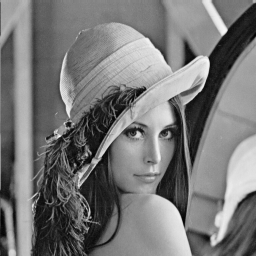
\includegraphics[width=.3\textwidth]{img_lena.png}} \hspace{30px}
\subfloat[Haar Transformed Image]{\label{fig:10-1b}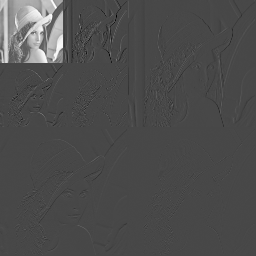
\includegraphics[width=.3\textwidth]{my_lena_haar_2.png}}
\caption{}
\label{fig:10-1}
\end{figure}

I performed a discrete Haar wavelet transformation to the image of Lena provided in \ttt{img\_lena.tif} using the algorithm presented in class, which used discrete sums and differences of neighboring pixels. The output takes on a reconstructed quadtree form, and shows two levels of wavelet decomposition.

\lstinputlisting{problem1.py}

\section{Problem 2}
\textbf{Why do the detail images in the wavelet transform enhance horizontal, vertical, and diagonal edges?}\\
To understand the detail images it is helpful to consider creating them by consecutively performing two 1D discrete wavelet transforms in each principal direction in the image. The output of the each pass of the 1D DWT returns two components of the input image, \ttt{cL} and \ttt{cH} which are the low and high frequency components of the image with respect to the decomposition wavelet used. In the case of the Haar wavelet, these components are simply the normalized sums and differences of neighboring pixels.

If the 1D DWT is run across horizontal pixels, then horizontal borders are in the direction of the pass, and therefore comprise a part of the \ttt{cL1} signal since the difference of neighboring pixels along a horizontal border is small.  Because vertical and diagonal borders are not in the same direction as the pass, the differences of neighboring pixels along the pass will be high at a vertical or diagonal border, and these borders will be contained in the \ttt{cH1} output of the 1D DWT.

In the second pass, both the \ttt{cL1} and \ttt{cH1} output of the first pass are run through the 1D DWT algorithm again, but in the vertical direction. When the \ttt{cL1} image is run through a vertical DWT, horizontal borders will now be perpendicular to the pass, and will appear as a part of the \ttt{cH2} output of this run.  The low frequency output \ttt{cL2} will then just be a smoothed version of the original image. When the \ttt{cH1} image is run through the vertical DWT, vertical borders will be along the pass, and will therefore constitute low frequency signals, output in \ttt{cL3}. Diagonal borders, on the other hand, will stil not be in the direction of the pass, and will be contained in the high frequency output \ttt{cH3}.

In this way, the output of the DWT consists of four images, \ttt{cL2}, \ttt{cH2}, \ttt{cL3}, \ttt{cH3}. Furthermore the detail images (all but \ttt{cL2}) represent enhanced horizontal, vertical, and diagonal boundaries of the original image.

\section{Appendix: Common Code}
The base code used for Problem 1 in this homework is contained in \ttt{mywavelet.py}.
\lstinputlisting{mywavelet.py}
\end{document} 
